\chapter{Questionário de Avaliação} %Apendice B
\label{apendice:b_quest_avaliacao}
\textit{A primeira questão é destinada a separar os grupos de respondentes de instituições sem PDTI e com PDTI:}
\\
\\1 - Sua instituição possui um Plano Diretor de TI (PDTI)? (Sim ou Não)
\\Resultado (32 respostas no total): 
\\Sim: 90,6\% (29 respostas); Não:9,4\% (3 respostas).

\textit{As perguntas a seguir foram destinadas ao grupo que respondeu "não" na questão 1:}
\\
\\1.1 - A área de TI da minha instituição é percebida como uma área estratégica para a instituição como um todo. (Escala de 1 a 5, onde 1 indica "discordo totalmente" e 5 "concordo totalmente").
\\Resultado:
\begin{figure}[h]
\centering % para centralizarmos a figura
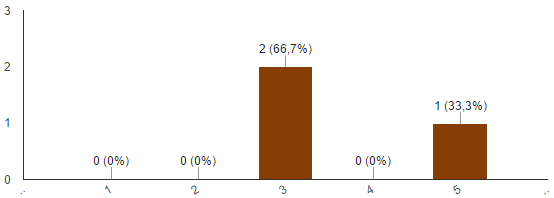
\includegraphics[width=10cm, frame]{figuras/apendiceB-1-2.png}
%\label{figura:grafico_ava_grupoSemPDTI}
%\caption{Aderência à teoria sobre as razões da ausência de um PDTI}
\end{figure}
\\
\\1.2 - A área de TI da minha instituição possui gestores que dominam técnicas e conceitos de nível estratégico na área (Governança de TI). (Escala de 1 a 5, onde 1 indica "discordo totalmente" e 5 "concordo totalmente").
\\Resultado:
\begin{figure}[h]
\centering % para centralizarmos a figura
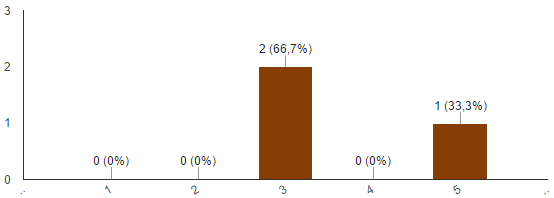
\includegraphics[width=10cm, frame]{figuras/apendiceB-1-2.png}
\end{figure}

\textit{A questão a seguir avalia a aderência da teoria fundamentada nos dados para as instituições sem PDTI:}
\\
\\1.3 - Uma instituição com baixo nível de maturidade em gestão não dá a devida importância à planos estratégicos e não reconhece a TI como parte estratégica da instituição. A área de TI, por sua vez, apresenta deficiências estratégicas como (a) baixo nível de influência da TI na instituição como um todo e (b) equipe inadequada em quantidade e em domínio de técnicas de planejamento; tais fatores (fator “a” e fator “b”) impedem ou dificultam a elaboração do Plano Diretor de TI.
\\Resultado (Escala de 1 a 5, onde 1 indica "discordo totalmente" e 5 "concordo totalmente"):
\begin{figure}[h]
\centering % para centralizarmos a figura
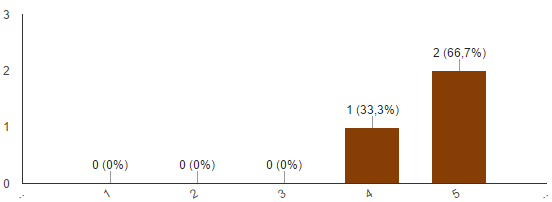
\includegraphics[width=10cm, frame]{figuras/grafico_ava_grupoSemPDTI.PNG}
\end{figure}

\textit{As perguntas a seguir foram destinadas ao grupo que respondeu "não" na questão 1:}
\\
\\2.1 - A participação dos setores, ou seja, das áreas de negócio no PDTI da minha instituição ocorreu com comprometimento e envolvimento satisfatórios. (Escala de 1 a 5, onde 1 indica "discordo totalmente" e 5 "concordo totalmente").
\\Resultado:
\begin{figure}[h]
\centering % para centralizarmos a figura
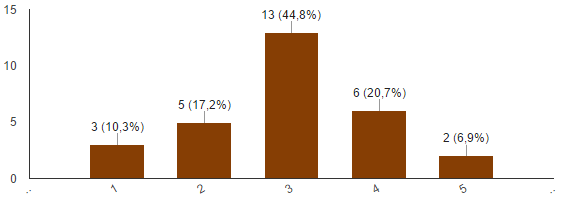
\includegraphics[width=10cm, frame]{figuras/apendiceB-2-1.png}
\end{figure}

\textit{A questão a seguir avalia a aderência da teoria fundamentada nos dados para as instituições sem PDTI:}
\\
\\2.2 - Uma determinada instituição apresenta o seguinte cenário: (a) possui membros que colocam interesses particulares e políticos acima dos interesses da instituição; (b) não possui a percepção de que a TI é parte estratégica e (c) não possuem recursos humanos devidamente capacitados para promover a cultura do planejamento. O efeito causado por (a), (b) e (c) no PDTI da instituição é a "falta de comprometimento e a participação insatisfatória das áreas de negócio" na composição do planejamento de TI. Esta atuação deficiente das áreas de negócio é o principal fator das dificuldades e deficiências encontradas na elaboração de um PDTI.
\\Resultado (Escala de 1 a 5, onde 1 indica "discordo totalmente" e 5 "concordo totalmente"):
\begin{figure}[h]
\centering % para centralizarmos a figura
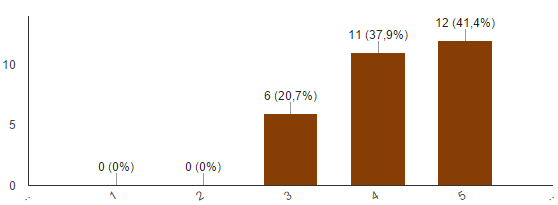
\includegraphics[width=10cm, frame]{figuras/grafico_ava_grupoComPDTI.PNG}
\end{figure}